
\begin{correction}  \;
\begin{enumerate}
\item  \textbf{R\'esolution de $\mathbf{ \tan^2{x}+(1-\sqrt{3})\tan{x}-\sqrt{3}=0 }$:}
Le domaine de d\'efinition est ici celui de la tangente, donc $\mathcal{D} = \R \backslash \left\{\ddp \frac{\pi}{2}+k\pi, k \in \Z\right\}$.
On pose alors $X=\tan{x}$.
On obtient
$$
\tan^2{x}+(1-\sqrt{3})\tan{x}-\sqrt{3}=0\Leftrightarrow 
\left\lbrace\begin{array}{l}
\tan{x}=X\vsec\\
X^2+(1-\sqrt{3})X-\sqrt{3}=0.
\end{array}\right.$$
On calcule le discriminant, en utilisant l'astuce qui consiste \`a ne pas rassembler les termes sans racine pour reconna\^itre une identit\'e remarquable : $\Delta=1+3+2\sqrt{3}=(\sqrt{3}+1)^2.$ On obtient donc $-1$ et $\sqrt{3}$ comme racines. Ainsi on se ram\`ene aux deux \'equations fondamentales suivantes:
$$
\tan^2{x}+(1-\sqrt{3})\tan{x}-\sqrt{3}=0\Leftrightarrow
\left\lbrace\begin{array}{l}
\tan{x}=-1\vsec\\
\hbox{ou}\vsec\\
\tan{x}=\sqrt{3}.
\end{array}\right.
\Leftrightarrow
%\left\lbrace\begin{array}{l}
%\tan{x}=\tan{\left( -\ddp\frac{\pi}{4}\right)}\vsec\\
%\hbox{ou}\vsec\\
%\tan{x}=\tan{\left(\ddp\frac{\pi}{3}\right)}.
%\end{array}\right.
\left\lbrace\begin{array}{l}
\exists k\in\Z,\ x=-\ddp\frac{\pi}{4}+k\pi\\
\hbox{ou}\\
\exists k\in\Z,\ x=\ddp\frac{\pi}{3}+k\pi.\\
\end{array} \right.
$$
\begin{minipage}[c]{0.45\textwidth}
On obtient ainsi: 
$$\fbox{$\mathcal{S}=\left\lbrace x=-\ddp\frac{\pi}{4}+k\pi,\ k\in\Z\right\rbrace\cup\left\lbrace \ddp\frac{\pi}{3}+k\pi,\ k\in\Z\right\rbrace$}.$$
\end{minipage}
\quad \begin{minipage}[c]{0.45\textwidth}
\begin{center}
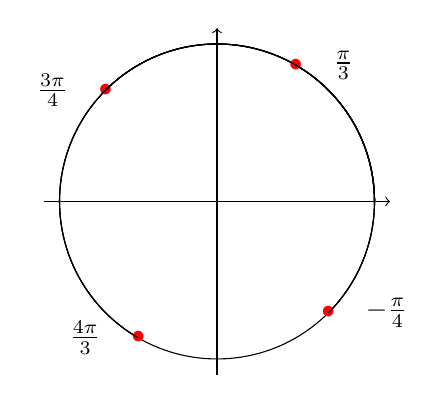
\begin{tikzpicture}[scale=2]
%Axes
\draw [->] (-1.1,0) -- (1.1,0);
\draw [->] (0,-1.1) -- (0,1.1);
%Cercle
\draw (0,0) circle (1);
%Points
\draw (1,0) arc (0:-45:1) node [red] {$\bullet$};
\draw (1,0) arc (0:-45:1) node[right] {$\quad \ddp -\frac{\pi}{4}$} ;
\draw (1,0) arc (0:135:1) node [red] {$\bullet$};
\draw (1,0) arc (0:135:1) node[left] {$\ddp \frac{3\pi}{4} \quad$} ;
\draw (1,0) arc (0:60:1) node [red] {$\bullet$};
\draw (1,0) arc (0:60:1) node[right] {$\quad \ddp \frac{\pi}{3}$} ;
\draw (1,0) arc (0:240:1) node [red] {$\bullet$};
\draw (1,0) arc (0:240:1) node[left] {$\ddp \frac{4\pi}{3}\quad$} ;
\end{tikzpicture}
\end{center}
\end{minipage}
%-----------------------------------------------------------------
\item  \textbf{R\'esolution de $\mathbf{ \sqrt{2}\sin^2{x}+(\sqrt{2}-1)\cos{x}+1-\sqrt{2}=0}$:}
On commence par transformer le sinus au carr\'e par un cosinus au carr\'e et on refait ensuite un raisonnement analogue.
L'\'equation \`a r\'esoudre devient alors
$$\begin{array}{lll}
\sqrt{2}\sin^2{x}+(\sqrt{2}-1)\cos{x}+1-\sqrt{2}=0&\Leftrightarrow  & \sqrt{2}\cos^2{x}+(1-\sqrt{2})\cos{x}-1=0\vsec\\
&\Leftrightarrow & 
\left\lbrace\begin{array}{l}
\cos{x}=X\vsec\\
\sqrt{2}X^2+(1-\sqrt{2})X-1=0.
\end{array}\right.\end{array}$$
La r\'esolution de l'\'equation du second degr\'e donne $\ddp\frac{-1}{\sqrt{2}}$ et $1$ comme racines. L\`a encore, il faut remarquer que: $\Delta=1+2+2\sqrt{2}=(1+\sqrt{2})^2.$
Ainsi on se ram\`ene aux deux \'equations fondamentales suivantes
$$
\sqrt{2}\sin^2{x}+(\sqrt{2}-1)\cos{x}+1-\sqrt{2}=0\Leftrightarrow  
\left\lbrace\begin{array}{l}
\cos{x}=-\ddp\frac{1}{\sqrt{2}}\vsec\\
\hbox{ou}\vsec\\
\cos{x}=1
\end{array}\right.
\Leftrightarrow 
\left\lbrace\begin{array}{l}
\cos{x}=\cos{\left( \ddp\frac{3\pi}{4} \right)}\vsec\\
\hbox{ou}\vsec\\
\cos{x}=\cos{(0)}
\end{array}\right.
$$
On obtient ainsi:
$$\fbox{$\mathcal{S}=\left\lbrace \ddp\frac{3\pi}{4}+2k\pi,\ k\in\Z\right\rbrace\cup\left\lbrace -\ddp\frac{3\pi}{4}+2k\pi,\ k\in\Z\right\rbrace\cup\left\lbrace 2k\pi,\ k\in\Z\right\rbrace$}.$$
\begin{center}
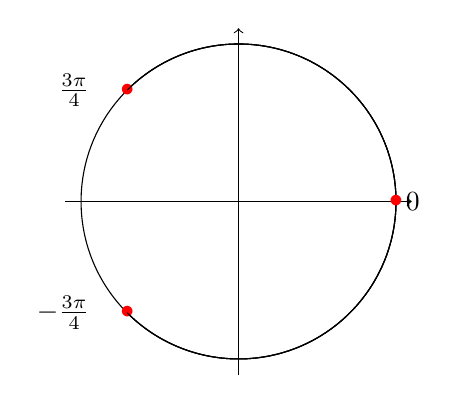
\begin{tikzpicture}[scale=2]
%Axes
\draw [->] (-1.1,0) -- (1.1,0);
\draw [->] (0,-1.1) -- (0,1.1);
%Cercle
\draw (0,0) circle (1);
%Points
\draw (1,0) arc (0:135:1) node [red] {$\bullet$};
\draw (1,0) arc (0:135:1) node[left] {$\ddp \frac{3\pi}{4} \quad$} ;
\draw (1,0) arc (0:-135:1) node [red] {$\bullet$};
\draw (1,0) arc (0:-135:1) node[left] {$\ddp -\frac{3\pi}{4} \quad$} ;
\draw (1,0) arc (0:0:1) node [red] {$\bullet$};
\draw (1,0) arc (0:0:1) node[right] {$\ddp 0$} ;
\end{tikzpicture}
\end{center}
%-----------------------------------------------------------------
\item  \textbf{R\'esolution de $\mathbf{ 2\sin^4{x}-\sin^3{x}-2\sin^2{x}+\sin{x}=0 }$:}
On fait l\`{a} encore un changement de variable. L'\'equation \`a r\'esoudre devient alors
$$\begin{array}{lll}
2\sin^4{x}-\sin^3{x}-2\sin^2{x}+\sin{x}=0
&\Leftrightarrow & 
\left\lbrace\begin{array}{l}
\sin{x}=X\vsec\\
2X^4-X^3-2X^2+X=0.
\end{array}\right.\end{array}$$
On obtient ainsi une \'equation de degr\'e 4, il faut donc commencer par rechercher les racines \'evidentes. On a tout de suite que 0 est racine \'evidente et on obtient alors que: $2X^4-X^3-2X^2+X=X(2X^3-X^2-2X+1)$. On remarque aussi que 1 est racine \'evidente ainsi que -1. On obtient donc que: $X(2X^3-X^2-2X+1)=X(X-1)(X+1)(aX+b)$. Puis par identification des coefficients d'un polyn\^{o}me, on obtient que: $2X^4-X^3-2X^2+X=X(X-1)(X+1)(2X-1)$. Ainsi les racines sont $-1$, $0$, $\ddp\demi$ et 1. On se ram\`{e}ne donc aux \'equations fondamentales suivantes:
$$
2\sin^4{x}-\sin^3{x}-2\sin^2{x}+\sin{x}=0\Leftrightarrow  
\sin{x}=-1 \; \hbox{ou} \; \sin{x}=0 \; \hbox{ou} \; \sin{x}=\ddp\demi \; \hbox{ou}\; \sin{x}=1.
$$
On obtient ainsi:
$$\fbox{$\mathcal{S}=\left\lbrace \ddp\frac{\pi}{2}+k\pi,\ k\in\Z\right\rbrace\cup\left\lbrace k\pi,\ k\in\Z\right\rbrace\cup\left\lbrace\ddp\frac{\pi}{6}+2k\pi,\ k\in\Z\right\rbrace\cup\left\lbrace\ddp\frac{5\pi}{6}+2k\pi,\ k\in\Z\right\rbrace$}.$$
\begin{center}
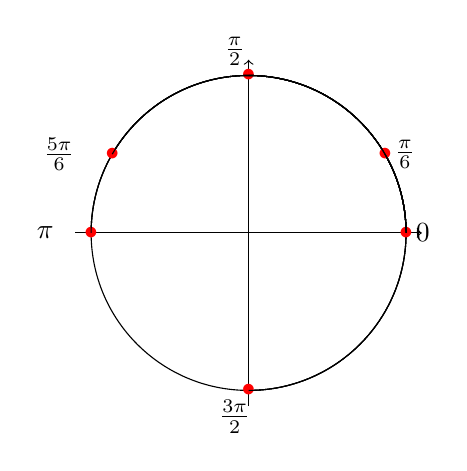
\begin{tikzpicture}[scale=2]
%Axes
\draw [->] (-1.1,0) -- (1.1,0);
\draw [->] (0,-1.1) -- (0,1.1);
%Cercle
\draw (0,0) circle (1);
%Points
\draw (1,0) arc (0:90:1) node [red] {$\bullet$};
\draw (1,0) arc (0:90:1) node[above] {$\ddp \frac{\pi}{2} \quad$} ;
\draw (1,0) arc (0:-90:1) node [red] {$\bullet$};
\draw (1,0) arc (0:-90:1) node[below] {$\ddp \frac{3\pi}{2} \quad$} ;
\draw (1,0) arc (0:180:1) node [red] {$\bullet$};
\draw (1,0) arc (0:180:1) node[left] {$\ddp \pi \quad$} ;
\draw (1,0) arc (0:0:1) node [red] {$\bullet$};
\draw (1,0) arc (0:0:1) node[right] {$\ddp 0$} ;
\draw (1,0) arc (0:30:1) node [red] {$\bullet$};
\draw (1,0) arc (0:30:1) node[right] {$\ddp \frac{\pi}{6}$} ;
\draw (1,0) arc (0:150:1) node [red] {$\bullet$};
\draw (1,0) arc (0:150:1) node[left] {$\ddp \frac{5\pi}{6} \quad$} ;
\end{tikzpicture}
\end{center}
\end{enumerate}
\end{correction}